% Well-motivated project with success criteria well-justified.

\label{sec:introduction}
Visual Simultaneous Localization and Mapping (visual SLAM) serves as the foundation of countless modern technologies, with self-driving cars, augmented reality devices, and autonomous drones just being a few examples. By using purely visual inputs, visual SLAM is able to create a 3D map of the surroundings while also localizing the camera's position within this map in real-time.

Unlike other SLAM systems which may use an expensive and heavy sensor such as LIDAR, RGB-Depth cameras, or Radar, visual SLAM only requires the ubiquitous camera sensor, allowing the technology to be used in many commercial applications such as Google's ARCore\footnote[1]{\url{https://developers.google.com/ar/develop/fundamentals}}, Boston Dynamic's GraphNav system used on their robot Spot\footnote[2]{\url{https://support.bostondynamics.com/s/article/GraphNav-Technical-Summary}}, and several models of DJI quadcopters\footnote[3]{DOI: 10.1016/j.vrih.2019.09.002} making this a particularly practical field of research.

\section{Motivation}
\label{sec:motivation}
Multi-robot systems are becoming increasingly common as automation continues to grow in a variety of fields, such as self-driving cars, drone swarms, and warehouse robots. These systems require the agents to understand the world around them as well as their peer's locations within that world. This task is often achieved with technologies such as GPS or motion capture setups, however, not all environments have access to these systems. A few emerging examples include: \noparskip
\smallbreak

{
    \begin{itemize}[nosep]
        \item Search and rescue operations in large indoor systems, assisted by drone swarms.
        \item Self-driving cars in underground road networks.
        \item Multi-agent cave/subsea exploration.
    \end{itemize}
}

These are scenarios where multi-agent SLAM provides a compelling solution, as it enables us to build a map of an unknown environment and keep agents aware of their relative poses. However, the majority of existing multi-agent visual SLAM implementations are centralized systems, requiring the agents to maintain reliable communications with a central server in order to operate. This is extremely detrimental, as environments that do not have access to GPS or motion capture systems are also likely to have very poor communication channels – greatly limiting the use cases of these centralized multi-agent SLAM systems.

Naturally, this leaves us with distributed multi-agent visual SLAM systems that do not rely on a centralized management server, allowing the agents to be used in environments where network infrastructure may be lacking. Instead of a central node, the agents are able to communicate peer-to-peer when they come within close proximity to one another.

It is easy to see the broad-reaching use cases of such a system. Agents will be able to explore sections of the world independently or in small teams, sharing new world locations with their peers as they come into communication range using an ad-hoc network. Agents will be able to accurately determine their peer's locations when they are within communication range, allowing for collision avoidance and cooperative path planning.

\section{Project Overview}
\label{sec:project-overview}
In this project, I: \noparskip
{
    \begin{enumerate}
        \item Design and implement a novel distributed monocular visual SLAM system, capable of localization, relative pose estimation, and collaborative mapping, all while being tolerant to degraded network conditions and not reliant on any single leader agent.
        \item Evaluate the performance of my system on standardized datasets, \textbf{demonstrating its superior performance over comparable state-of-the-art systems}.
        \item Create a simulation environment for testing and evaluating my system locally.
        \item Deploy my system on physical robots, \textbf{demonstrating the practical use cases of this system and benchmarking real-world performance.}
        \item \textbf{Contribute as a co-author to the paper \textit{The Cambridge RoboMaster: An Agile Multi-Robot Research Platform}}, where my distributed SLAM system was used to evaluate the robotics platform.
        \item Additionally, \textbf{I was an author of the paper \textit{The Cambridge RoboMaster: An Agile Multi-Robot Research Platform}}, with my distributed SLAM system included as one of the experiments analyzed in the paper.
        \item Develop \textit{Multi-Agent EVO} – the first open-source evaluation library for multi-agent SLAM systems.
        \item Develop the \textit{Raspberry Pi Video Publisher} – a performant platform for SLAM data collection or augmented reality visualizations – and set up a continuous integration and deployment pipeline to automatically push the latest build to the hardware.
    \end{enumerate}
}

\begin{leftbar}
    \textbf{A short video demonstration of my project is provided at the following URL:} \url{https://cam-diss.s3.amazonaws.com/video.mp4} \comment{TODO: fix video index} \captionbreak Due to the highly visual and 3D nature of my project, \textbf{I strongly recommend viewing the video}. It will provide an intuition of my system, making the following chapters easier to visualize and understand. Additionally, it is referenced throughout the dissertation.
\end{leftbar}

\begin{figure}[h]
    \centering
    \captionsetup{format=plain}
    \begin{subfigure}[t]{0.475\linewidth}
        \centering
        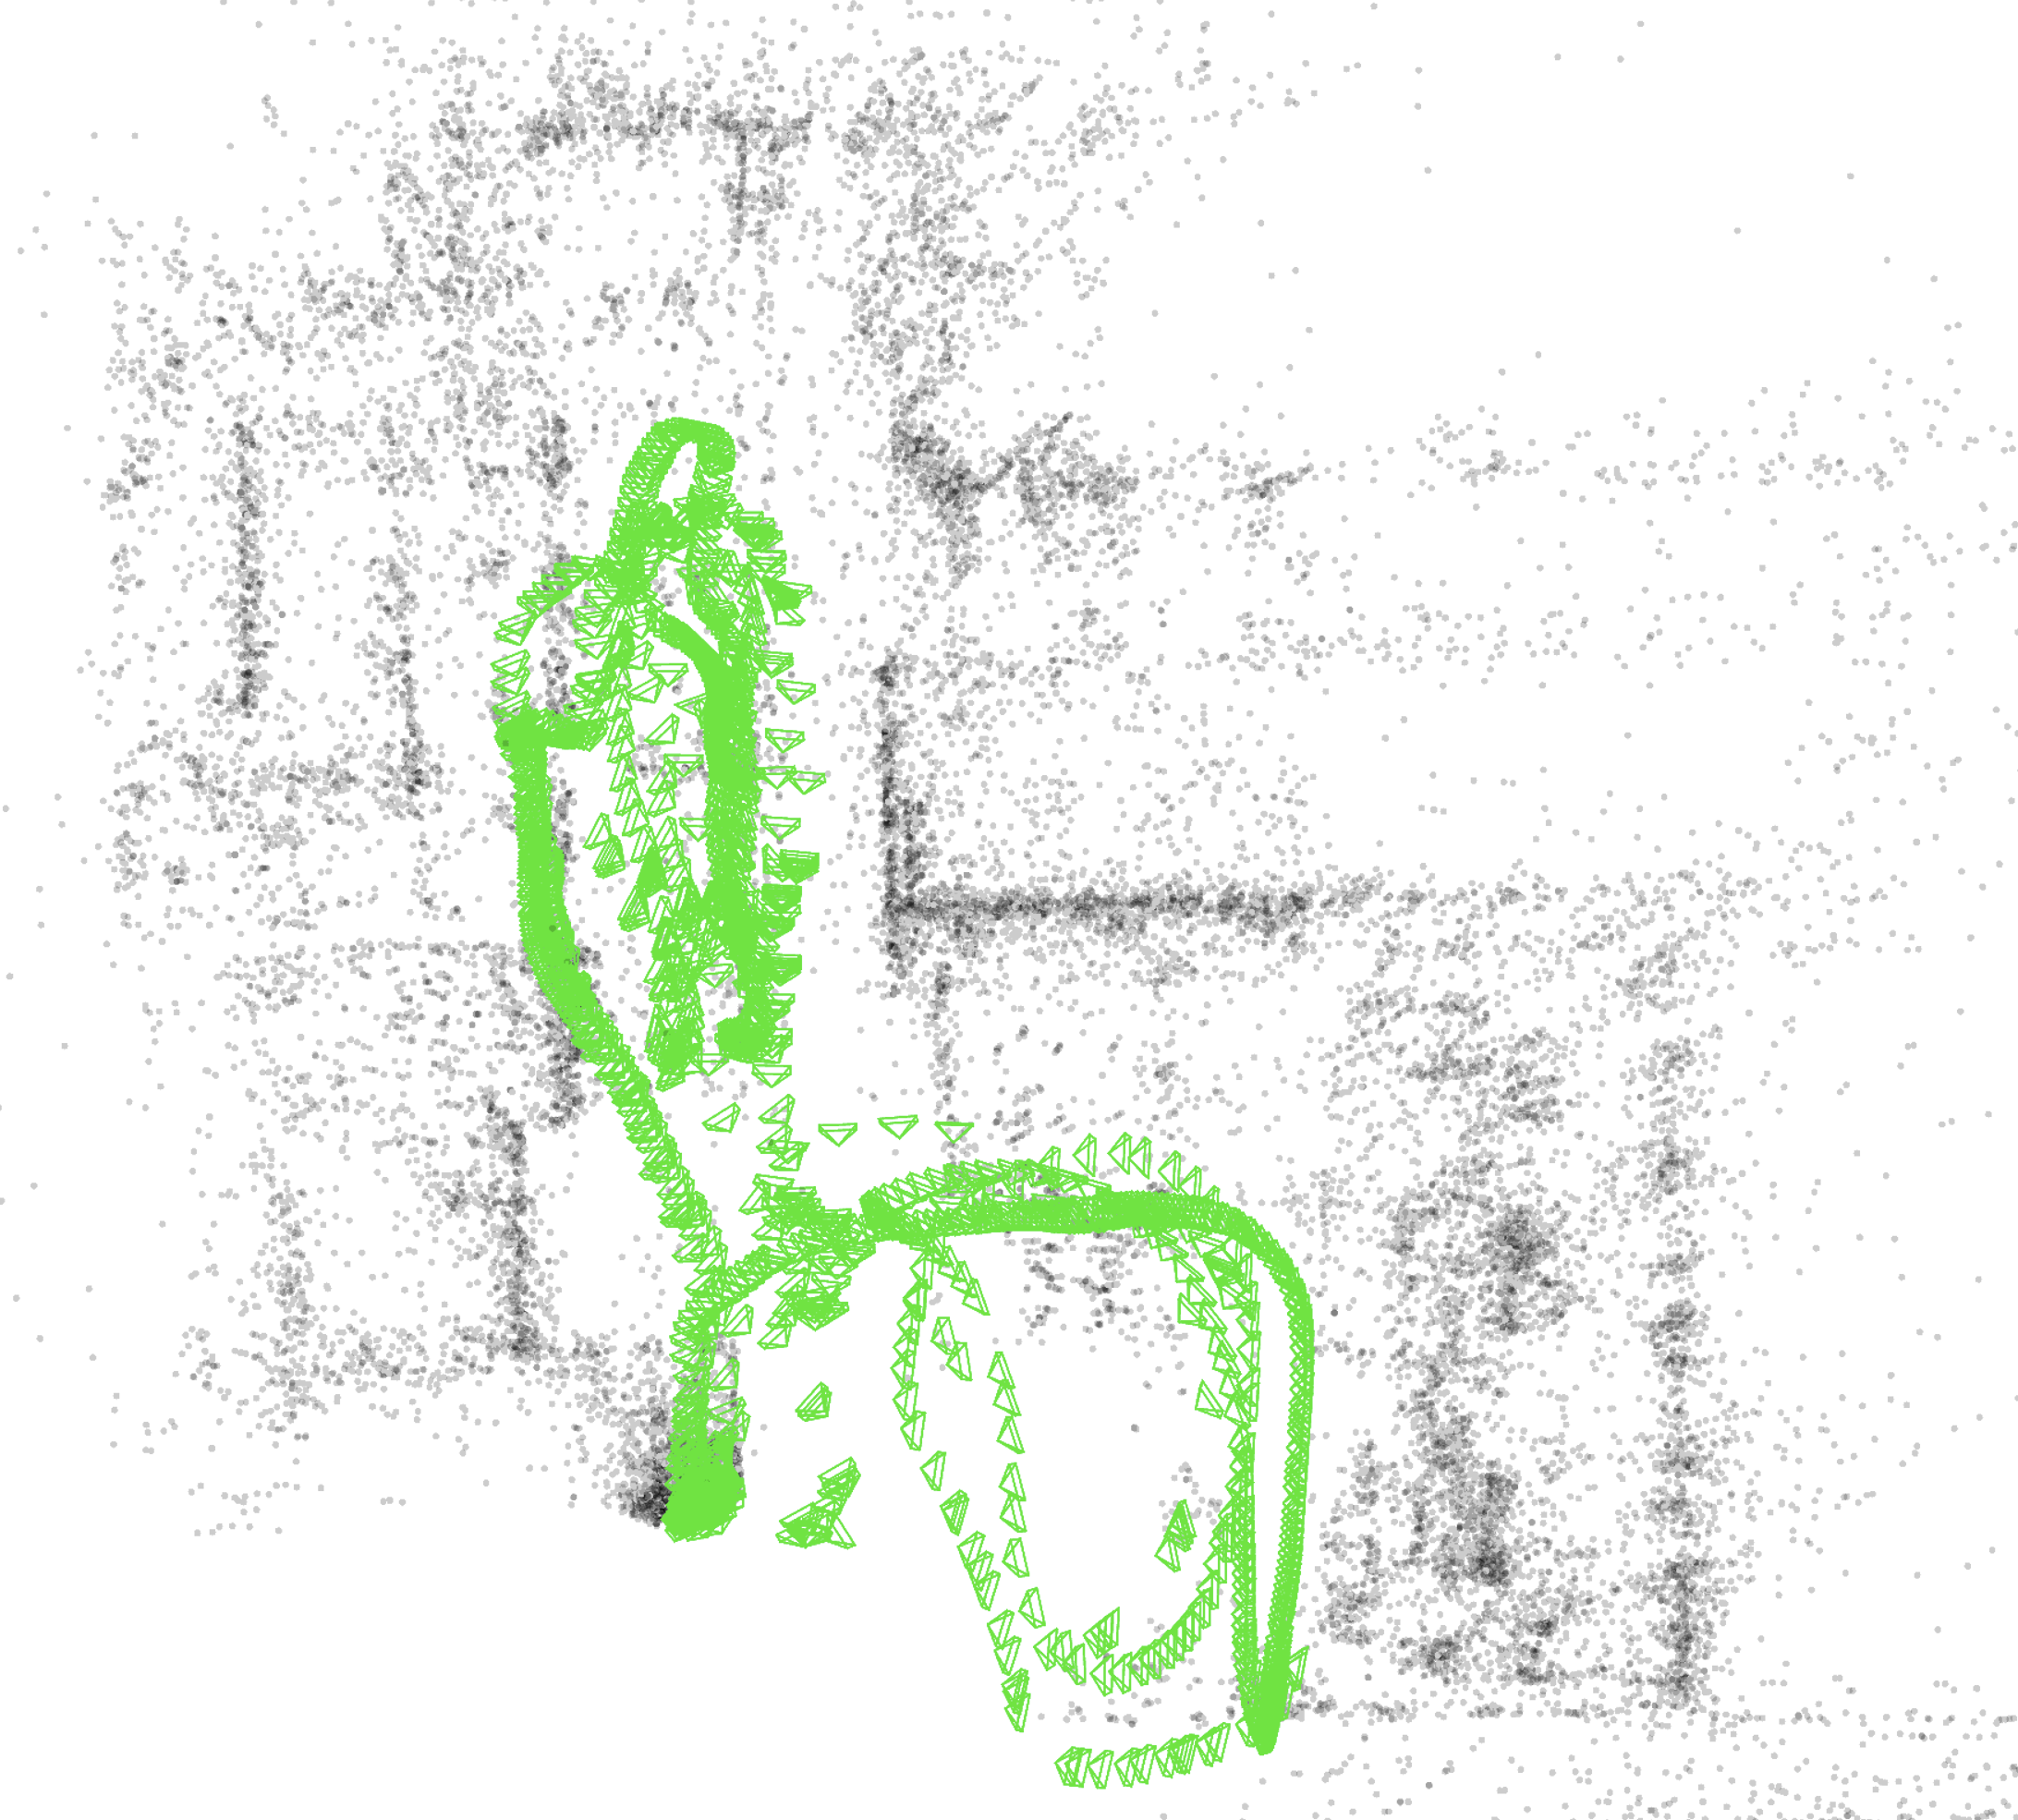
\includegraphics[height=2.2in]{figures/euroc_mh_map.png}
        \caption{EuRoC Machine Hall 01-03}
    \end{subfigure}\hfill%
    ~
    \begin{subfigure}[t]{0.475\linewidth}
        \centering
        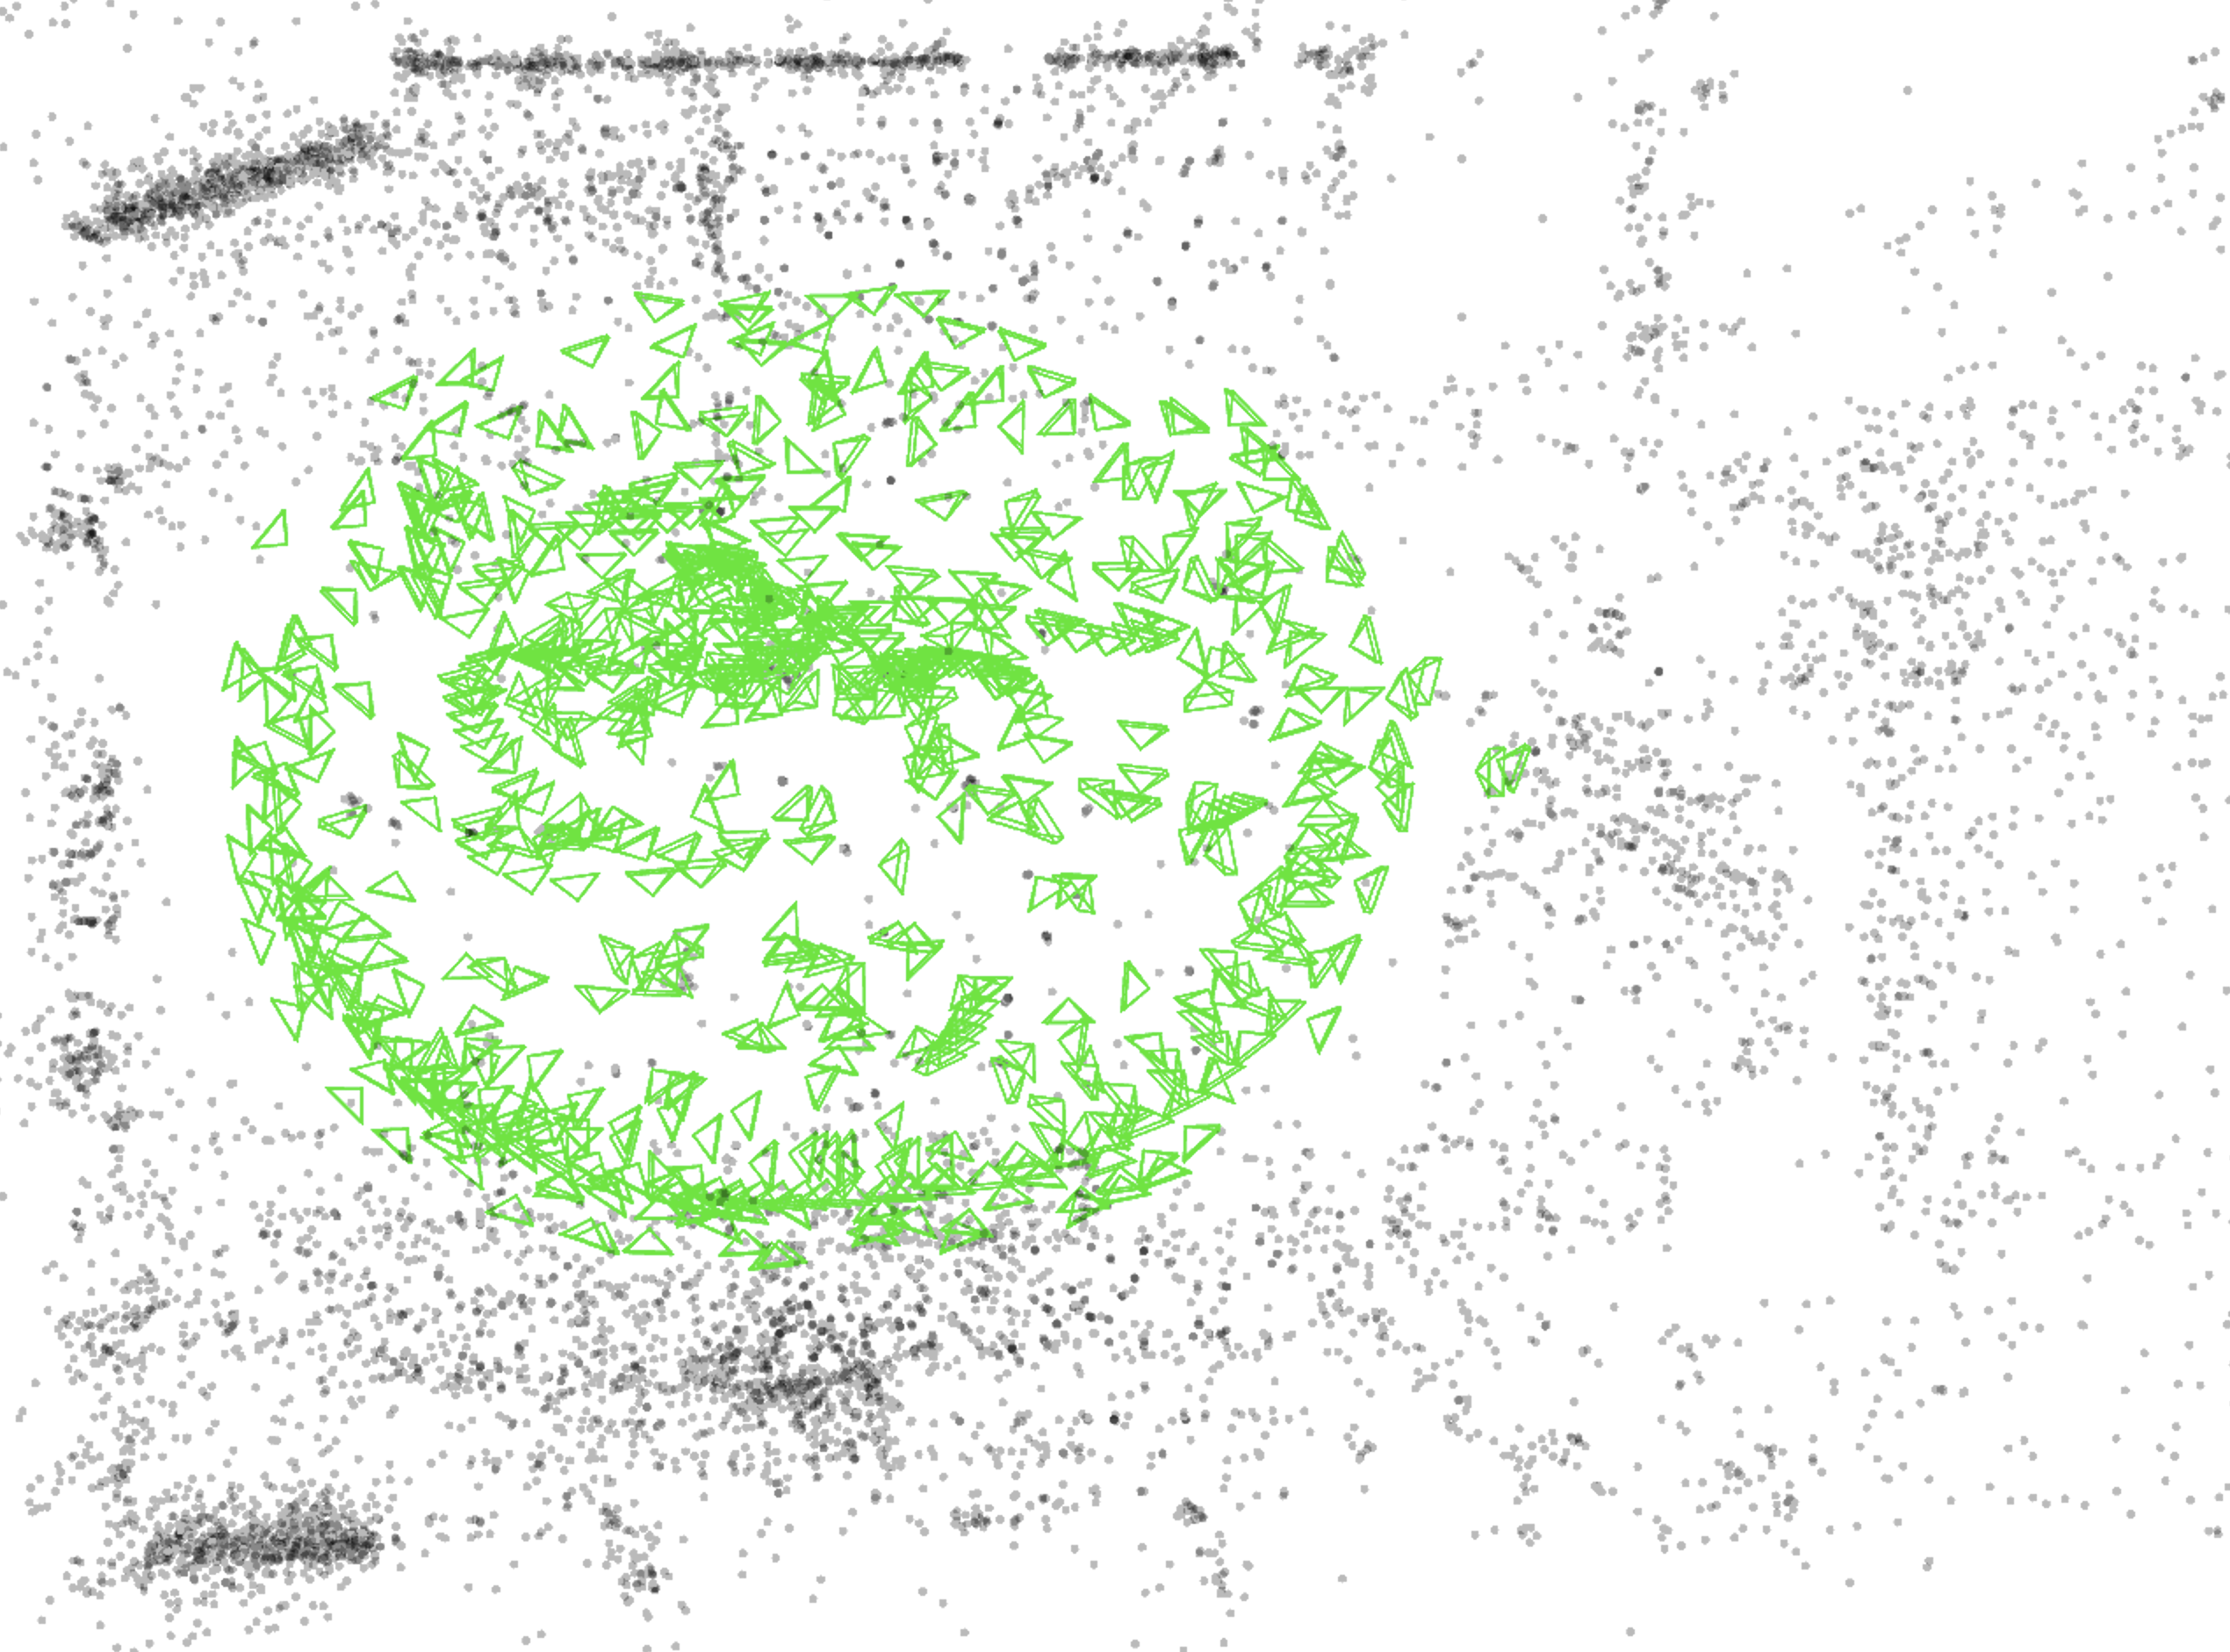
\includegraphics[height=2.05in]{figures/tum_room_map.png}
        \caption{TUM-VI Rooms 1-3}
    \end{subfigure}

    \caption{Sparse maps built by my distributed SLAM system running industry-standard datasets.}
    \label{fig:example-maps}
\end{figure}
